\newpage
\section{opercalc} \label{opercalc}

\subsection{General}
The program {\bf opercalc} calculates extrapolation operators for a given frequency. This program uses the same algorithm as is used in the programs \htmlref{{\bf extrap}}{extrap}, \htmlref{{\bf cfpmod}}{cfpmod} and \htmlref{{\bf migr}}{migr}. This program can be used to check whether the defined parameters for the calculation of the operator table are correct. It also showes how the different optimization algortihms distort the spatial-frequency spectrum of the extrapolation operator.

\subsection{Parameters}

Via the command-line or in a parameter file: {\tt par=$<$parameter\_file$>$}.
{\footnotesize
\begin{verbatim}
 opercalc - calculates extrapolation operators for a given frequency
 
 opercalc  file_out= [optional parameters] > Kx-file and X-file
 
 Required parameters:
 
   file_out= ................ base name of the output file(s)
 
 Optional parameters:
 
   freq=20 .................. frequency at which the operator is calculated
   c=2000 ................... velocity of the medium
   dx=15 .................... stepsize in spatial direction
   dz=dx .................... extrapolation step
   nkx=512 .................. number of kx samples
 EXTRAPOLATION OPERATOR DEFINITION 
   opl=25 ................... length of the convolution operator (odd)
   alpha=65 ................. maximum angle of interest
   perc=0.15 ................ smoothness of filter edge
   amp=0.5 .................. amplitude smooth operator
   weight=5e-5 .............. weight factor in WLSQ operator calculation
   filter=1 ................. using filter in kx-w domain before WLSQ
   beta=3 ................... 2 < beta < 10; factor for KAISER window
   nbw=3 .......... ......... order of butterworth filter
 OUTPUT DEFINITION 
   cycle=0 .................. 1; units along kx-axis set to 1.0/nkx
   on_su_pipe=0 ............. 1: x or 2: Kx results on SU-pipe
   verbose=0 ................ >0: shows various parameters and results
 
 The two files produced have a _x or _kx extension in the filename.
 The _x-file contains the optimized convolution operators (9x). 
 The _kx-file contains the spatial spectrum of the operators (10x):
         - 1 = Truncated operator
         - 2 = Gaussian tapered operator
         - 3 = Kaiser tapered operator
         - 4 = Smoothed Phase operator
         - 5 = Weighted Least Squares operator
         - 6 = Remez exchange operator
         - 7 = Hankel function H_1(2)
         - 8 = Non-linear CFSQP optimization
         - 9 = Smooth WLSQ operator
         - 10= Exact operator (phase shift)
 
  Copyright 1997, 2008 Jan Thorbecke, (janth@xs4all.nl) 
 
     intitial version   : 14-12-1993 (j.w.thorbecke@tudelft.nl)
          version 1.0   : 17-10-1995 (release version)
          version 2.0   : 23-06-2008 (janth@xs4all.nl) 2008
\end{verbatim}}
\noindent
{\bf NOTE:} This program can be run using the same parameter setup or parameter file as the other main programs of the EXTRAP directory.

\subsection{File formats}

The two files produced have a \_x or \_kx extension in the filename.
The x-file contains the optimized operators (7 traces) in the spatial domain.
The kx-file has 9 traces with trace number:

\hangindent=1.cm \hangafter=0
(1) Truncated operator \\ (2) Gaussian tapered operator \\ (3) Kaiser tapered operator \\  (4) Smoothed Phase operator \\ (5) Weighted least-squares \\ (6) Remez exchange operator \\ (7) Hankel function H$_1$(2) \\ (8) Non-linear CFSQP optimization \\ (9) smooth WLSQ operator \\ (10) Exact operator 

\subsection{General parameter description}

All are set to default values. The operators are computed in the wavenumber domain for all wavenumber values defined. The operators
are transformed back to the spatial domain, with or without an optimization step. The optimization is described  in Thorbecke (2004). Parameter {\tt nkx} defines the number of operator points in the wavenumber domain (double sided number). Parameter {\tt opl} defines the number of operator points in the space domain (double sided number, odd). Parameters {\tt dx} and and {\tt dz} define the spatial sampling intervals, parameter {\tt c} the velocity, {\tt freq} the frequency. The parameter {\tt alpha} defines the minimum and maximum angle of the extrapolation operators. The optimization using least-squares is controlled via the parameters {\tt weight}, {\tt alpha} and {\tt perc}.

The parameter {\tt alpha} defines the wavenumber window for which the optimization is carried out. The influence of the wavenumbers outside this window is taken to be less important. The importance of the wavenumbers outside the window is described by the parameter {\tt weight}. If {\tt weight=1} then all wavenumbers are equally important for the optimization and the 'optimized' result is in fact a truncation. For weighting values less than one the wavenumbers outside the wavenumber band of interest are less important. A very small weight factor can give rise to unstable results so in order to remain stable in the recursion a weight factor between 1.e-4 and 1e-7 is most convenient. The parameter {\tt perc} describes over which bandwidth the wavenumber spectrum is filtered. It is defined as the fraction of the band of interest over which the filtering is carried out.

The output is arranged via the parameters {\tt file\_out}, {\tt on\_su\_pipe} and {\tt cycle}.

\subsection{Examples}

To display the default operators just type:

{\footnotesize
\begin{verbatim}
opercalc on_su_pipe=2 file_out=nep.su | suamp | suxgraph style=normal
\end{verbatim}}

for the spectra of the convolution operators, to display the spatial convolution operators type:

{\footnotesize
\begin{verbatim}
opercalc on_su_pipe=1 file_out=nep.su | suamp | suxgraph style=normal
\end{verbatim}}

%
\begin{figure}[hb]
  \begin{pspicture}(8,5.2)
    \put(-0.5,-0.3){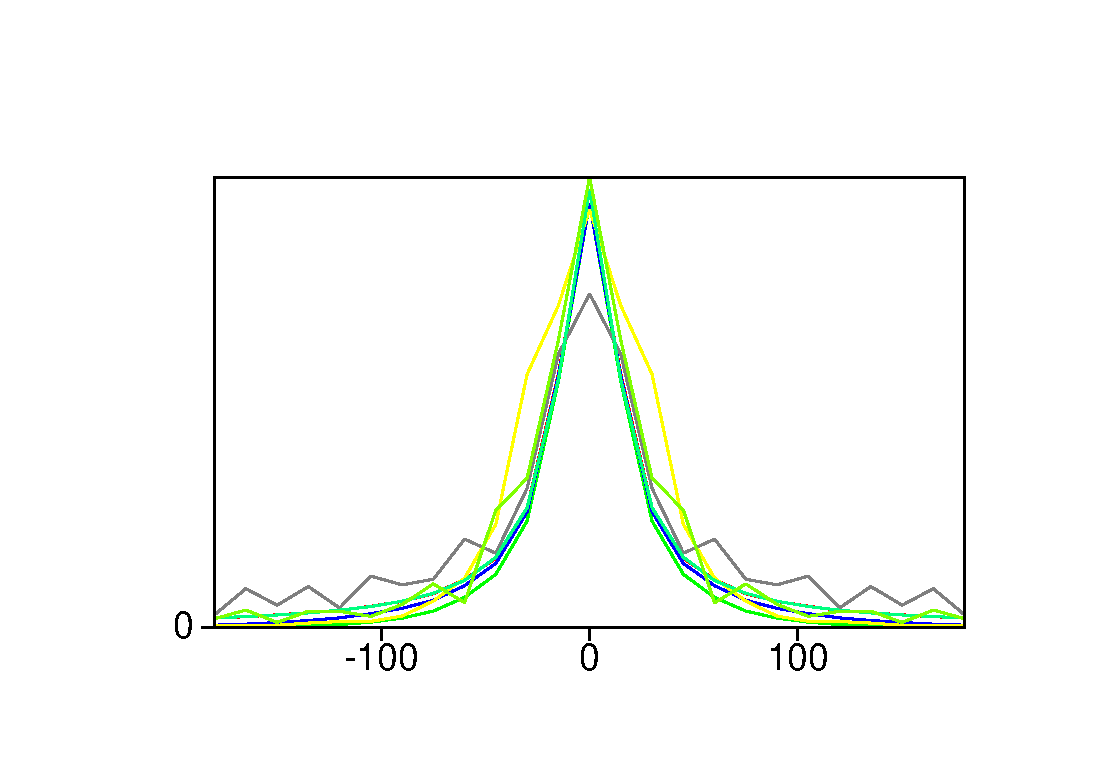
\epsfig{file=EPS/opercalc_x.eps,height=6cm}}
    \put(7.0,-0.3){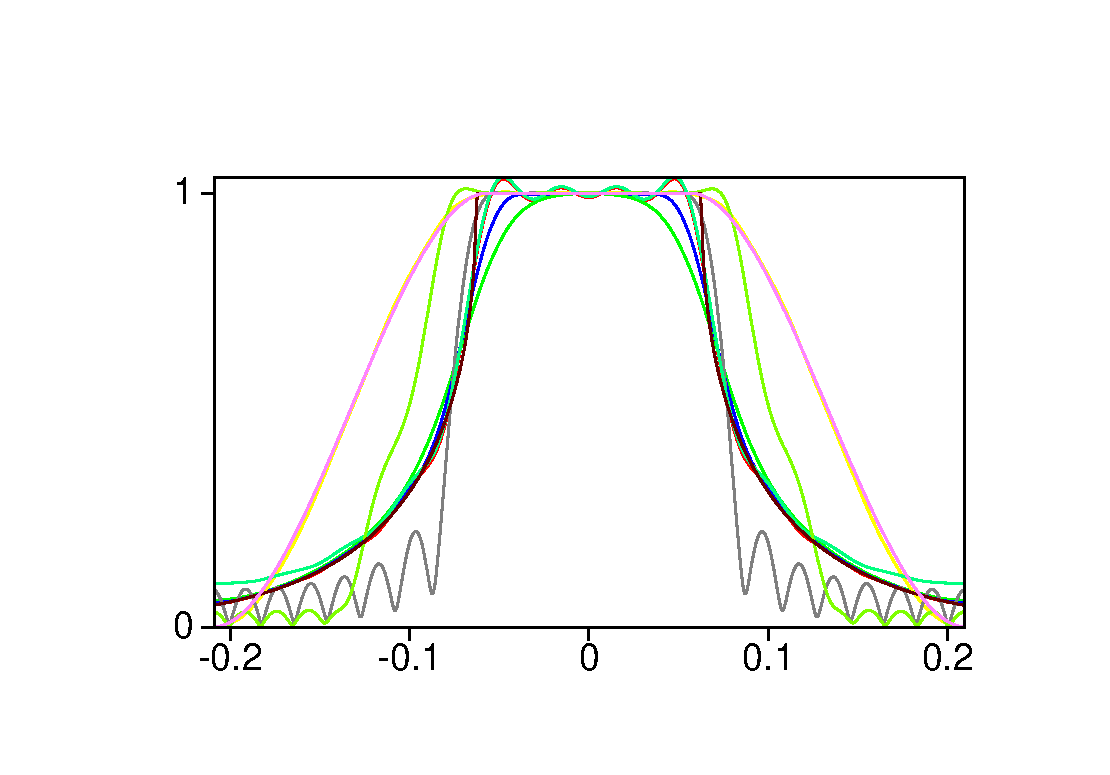
\epsfig{file=EPS/opercalc_kx.eps,height=6cm}}
\end{pspicture}
\caption{Wavefield extrapolation operators calculated by opercalc. Left shows the amplitude of the optimised operator in the spatial
domain and right shows the amplitude in the wavenumber domain. } \label{opercalc1}
\end{figure}


\subsection{To do}
Nothing really...
